\chapter{Evaluation}\label{ch:evaluation}

\section{Evaluationsziel und Untersuchungsdesign}
Ziel der Evaluation ist es, die in der vorliegenden Arbeit entwickelte Pipeline zur Generierung interaktiver Vivian-Prototypen systematisch zu untersuchen. Im Mittelpunkt steht dabei nicht die Bewertung der Bedienbarkeit durch externe Benutzer*innen, sondern die technische Funktionsfähigkeit des prototypisch umgesetzten Workflows. Daher wird die Evaluation als technische, szenariobasierte Systemevaluation durchgeführt. Sie prüft, ob aus den definierten Eingaben vollständige Vivian-Spezifikationen generiert werden können und ob das damit ermöglichte Verhalten dem zuvor festgelegten Referenzszenario entspricht.

In der Evaluation werden drei Aspekte betrachtet. Es wird geprüft, ob der VSG grundsätzlich in der Lage ist, aus vorhandenen 3D-Objekten ausführbare Prototypen zu erzeugen. Anschließend wird im zweiten Schritt bewertet, ob relevante Teilobjekte, Rollen, Zustände, und Übergänge wie erwartet aus dem Asset und der Interaktionsbeschreibung abgeleitet werden. Drittens wird schließlich untersucht, welchen Beitrag die Validierungs- und Korrekturmechanismen zur Verringerung von Fehlern leisten. Damit wird die Evaluation der in dieser Arbeit entwickelten Pipeline nicht nur auf einzelne Beispielausgaben reduziert, sondern betrachtet inhaltliche Qualität der erzeugten Vivian-Spezifikationen sowie die Robustheit des Workflows.

Zur Evaluation der in dieser Arbeit entwickelten Pipeline sollen verschiedene Assets systematisch getestet werden.
Es werden dazu drei Testassets mit unterschiedlicher Komplexität betrachtet: eine Lampe, ein Display und ein Toaster. Für jedes dieser Assets wird ein Szenario definiert, welches die erwarteten Teilobjekte, Rollen, Zustände, Übergänge und visuellen Reaktionen beschreibt. Da verschiedene valide Vivian-Spezifikationen dasselbe Verhalten abbilden können, bildet es einen verhaltensbezogenen Maßstab zur Bewertung, mit welchem schließlich die generierten Ergebnisse eingeordnet werden können.

Das Untersuchungsdesign beinhaltet qualitative sowie quantitative Bestandteile und ist entlang der Forschungsfragen aus~\ref{sec:forschungsfragen_zielsetzung} aufgebaut. Anhand eines Testassets wird zunächst untersucht, wie der VSG von Anfang bis Ende arbeitet und ob ein valider Vivian-Prototyp entsteht. Insbesondere die technische Umsetzbarkeit des Co-Creation-Workflows aus F1 wird damit adressiert. Die Bewertung erkannter Teilobjekte und zugewiesener Rollen bezieht sich auf die Frage, ob sich relevante Objekte, Teilobjekte und semantische Rollen aus vorhandenen Szeneninformationen und Nutzer*innenbeschreibungen ableiten lassen (F2). Die Untersuchung der abgeleiteten Interaktionslogik aus F3 wird mit der Analyse der erzeugten Zustände, Übergänge und visuellen Verhaltensänderungen adressiert. Es werden weiterhin wiederholte Durchläufe mit identischen Eingaben durchgeführt, um die Stabilität der Pipeline zu bewerten. Außerdem wird die vollständige Generierungspipeline mit einer Erstgenerierung ohne Korrekturschleife verglichen. Damit wird untersucht, ob Consistency Reviewer, Validator und Fixer Agent die Anzahl der Fehler reduzieren und die Erfolgsquote der finalen Vivian-Spezifikation erhöhen.

\section{Testassets und Referenzszenarien}

Zur Evaluation des VSG wurden drei Assets ausgewählt: eine Lampe, ein Display und ein Toaster.
Dabei steht nicht die Untersuchung einer möglichst großen Menge unterschiedlicher Objekte im Fokus, sondern eine gezielte Auswahl aussagekräftiger Beispiele. Diese ermöglicht es, die Funktionsfähigkeit des VSG über verschiedene Komplexitätsstufen sowie unterschiedliche Anforderungen zu prüfen. Die drei Assets dienen als Grundlage für eine szenariobasierte Evaluation, bei der die erzeugten Spezifikationen mit den zuvor festgelegten Verhaltenserwartungen als Referenz verglichen werden.

\begin{figure}[htbp]
  \centering
  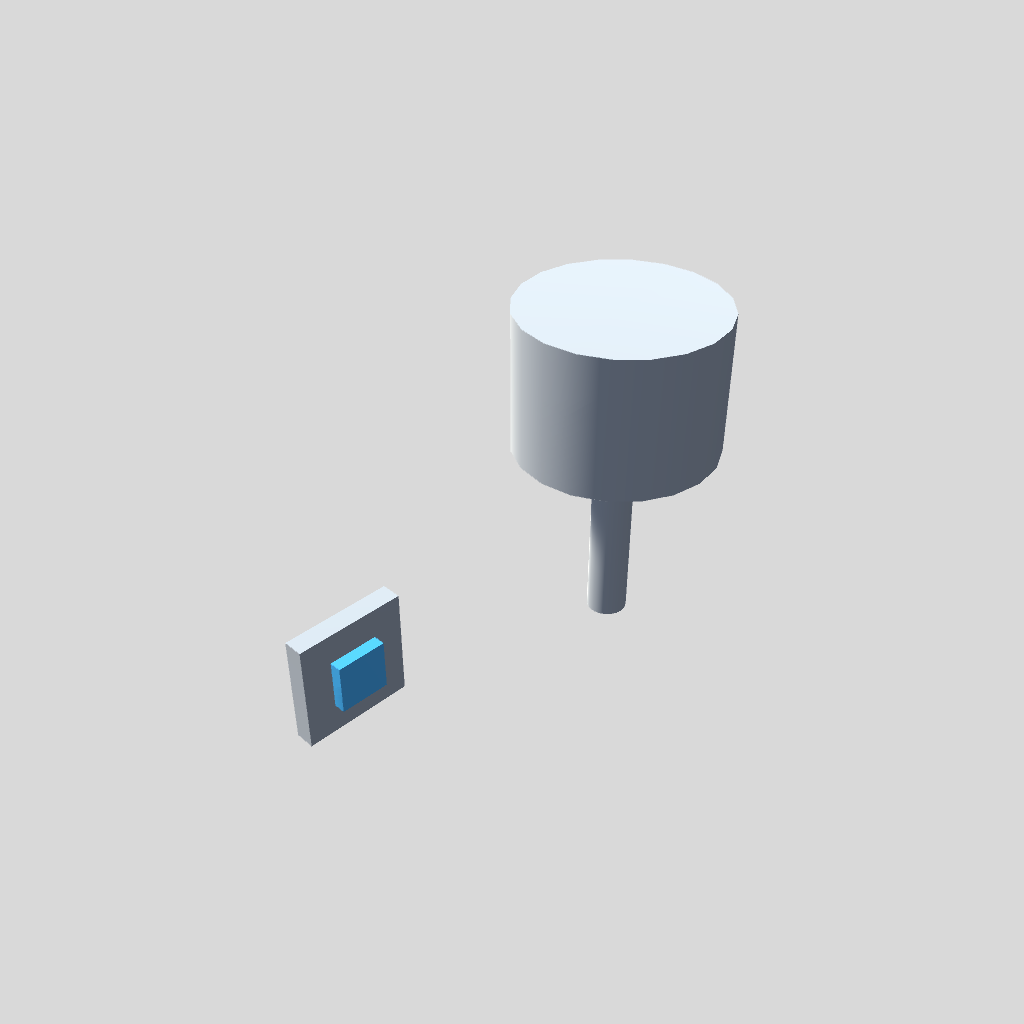
\includegraphics[width=0.3\linewidth]{figures/asset-examples-iso/Lamp_iso_top_right}\hfill
  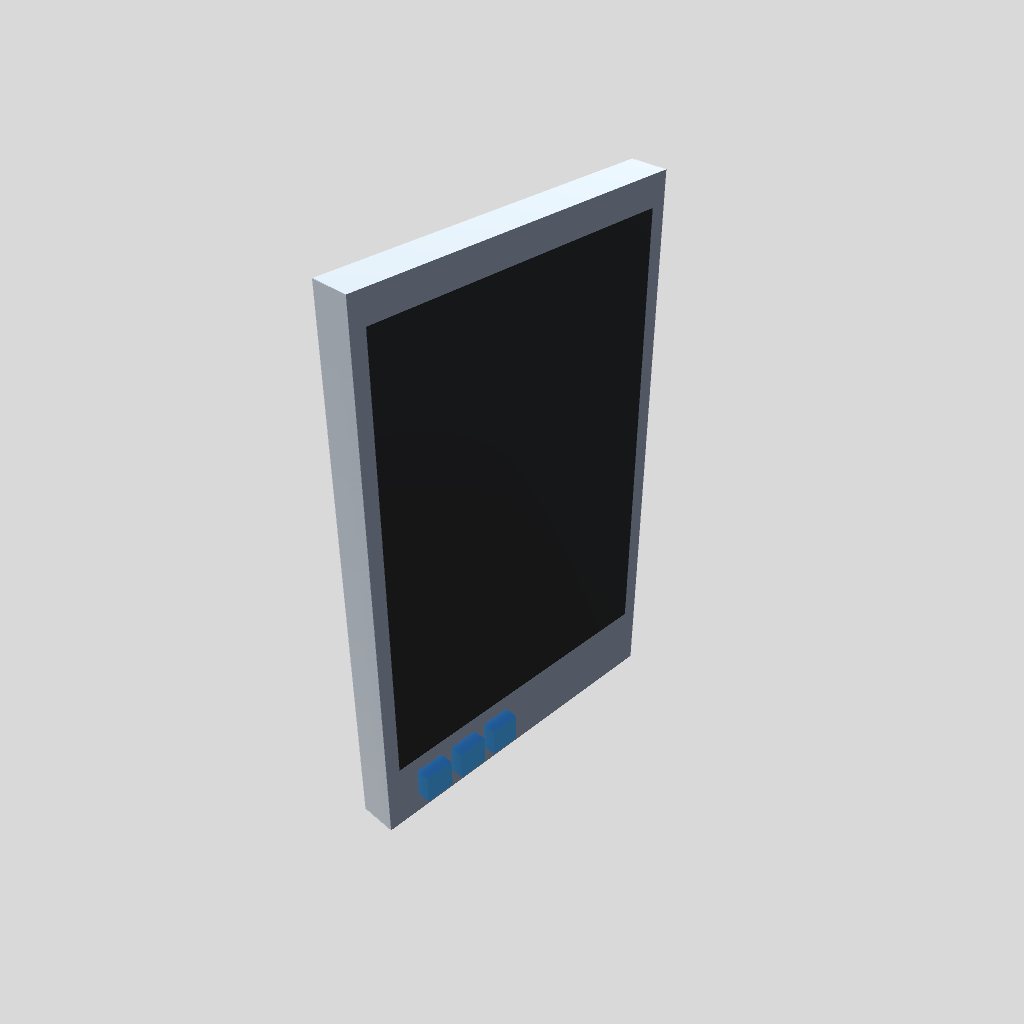
\includegraphics[width=0.3\linewidth]{figures/asset-examples-iso/Display_iso_top_right}\hfill
  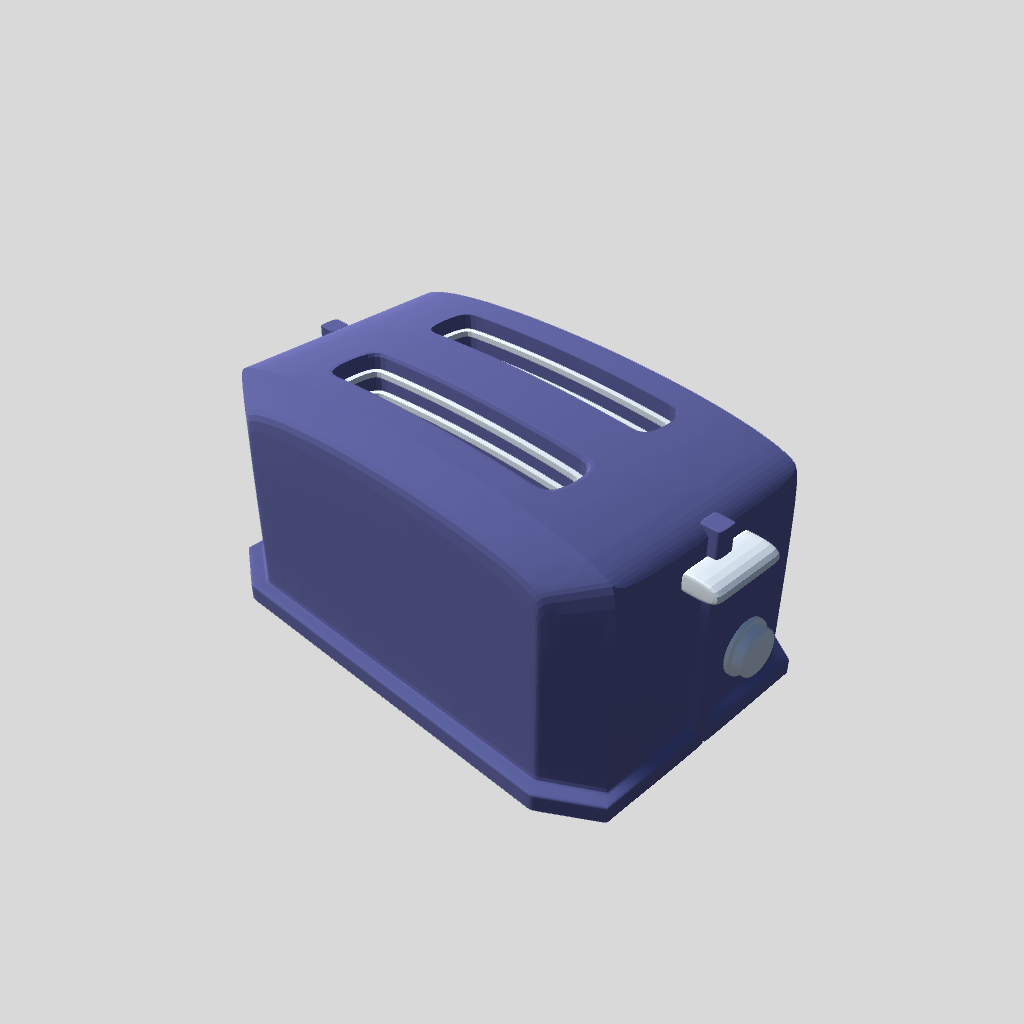
\includegraphics[width=0.3\linewidth]{figures/asset-examples-iso/toaster3_iso_top_right}
  \caption{Die drei Testassets Lampe, Display und Toaster (von links nach rechts).}\label{fig:testasset_examples_iso}
\end{figure}

Die drei Assets unterscheiden sich hinsichtlich ihrer funktionalen sowie strukturellen Komplexität, wodurch der Workflow nicht nur an einem einfachen Erfolgsbeispiel, sondern anhand verschiedener Testfälle mit steigender Komplexität und Anforderungen gezeigt werden kann. Die Lampe bildet das einfachste Beispiel ab, da hier nur eine Interaktion sowie eine visuelle Reaktion erwartet werden. Einen mittleren Schwierigkeitsgrad stellt das Display dar, da hier verschiedene Bedienelemente und eine Screen-Fläche erkannt sowie in Beziehung zueinander gesetzt werden müssen. Abschließend bietet der Toaster das komplexeste Beispiel, da hier mehrere Teilobjekte, unterschiedliche visuelle Rückmeldungen, verschiedene Zustände sowie ein zeitbasierter Übergang miteinander funktionieren müssen.

Für die Bewertung der Pipeline sind verschiedene Kriterien relevant, anhand derer die Auswahl der Testassets erfolgte. Ein erstes Kriterium ist die Auswahl relevanter Teilobjekte. Je mehr Teilobjekte ein Asset besitzt, desto anspruchsvoller ist für den VSG, jene Bestandteile zu identifizieren, die tatsächlich relevant für die gewünschte Interaktion sind. Bei der Lampe betrifft das den Knopf sowie den Lampenschirm bzw. die Lichtquelle. Beim Display hingegen müssen bereits mehrere Bedienelemente sowie eine Screen-Fläche erkannt und unterschieden werden. Das Toaster-Beispiel enthält zusätzlich einen Hebel, eine Stopp-Taste sowie Heizelemente zur Visualisierung.

Ein zweites Kriterium beschreibt die Anzahl und Art der erwarteten Rollen. Nicht nur muss die Pipeline relevante Objektbestandteile erkennen, sondern diese später auch passenden funktionalen Vivian-Rollen zuordnen. Während die Lampe mit zwei Arten von Interaktions- sowie Visualisierungselementen (\textit{Button} und \textit{Light}) auskommt, benötigt das Display neben mehreren Eingabeelementen (\textit{Buttons}) auch ein Screen-Element, um Inhalte tatsächlich anzuzeigen. Beim Toaster müssen unterschiedliche Rollen erkannt werden, wie Hebel und Stopp-Taste als Bedienelemente (\textit{Slider} und \textit{Button}) sowie visuelle Elemente wie LED und Heizelemente als \textit{Lights}.

Auch die Komplexität der Interaktionslogik stellt ein Auswahlkriterium dar. Weniger komplexe Prototypen kommen mit weniger komplexer Logik aus. Beim Lampen-Beispiel schaltet ein Knopfdruck das Licht an oder aus. Komplexere Prototypen wie das Display benötigen wiederum bereits mehrere voneinander unterscheidbare Aktionen. Ein Knopf schaltet das Display an oder aus und weitere Knöpfe ermöglichen ein Wechseln zwischen verschiedenen Seiten. Der Toaster enthält zudem eine zeitbasierte Komponente, welche es ermöglicht, einen Toastvorgang wahlweise per Tastendruck oder nach einer fest definierten Zeit zu beenden. Dieser Fall umfasst nach direkten Interaktionen somit auch eine automatische Zustandsänderung nach Ablauf einer definierten Zeit.
Außerdem wurden unterschiedliche visuelle Rückmeldungen berücksichtigt. Für die Evaluation ist dies wichtig, da ein Prototyp intern korrekt umgesetzte Zustände und Zustandsübergänge nachvollziehbar für Nutzer*innen veranschaulichen soll. Die Lampe verwendet dafür das Leuchten des Lampenschirms. Das Display-Beispiel nutzt die Darstellung der Screen-Inhalte und der Toaster simuliert das Glühen der Heizelemente sowie das Leuchten einer LED während des Toastvorgangs.

\begin{table}[htbp]
  \centering
  \begin{tabularx}{\linewidth}{ll>{\raggedright\arraybackslash}X}
    \toprule
    Asset   & Komplexität & Erwartete Hauptfunktion                                                                                                                                                 \\
    \midrule
    Lampe   & leicht      & Der Lampenschirm soll als Lichtquelle leuchten. Ein Knopf soll die Lampe an- \bzw ausschalten.                                                                          \\
    Display & mittel      & Das Display soll ein- und ausgeschaltet werden können, Screen-Inhalte anzeigen sowie zwischen Seiten wechseln können.                                                   \\
    Toaster & schwer      & Der Toastvorgang soll durch den Hebel gestartet, mittels LED und Heizelementen visualisiert sowie nach zehn Sekunden oder durch Drücken der Stopp-Taste beendet werden. \\
    \bottomrule
  \end{tabularx}
  \caption{Übersicht der ausgewählten Testassets.}\label{tab:übersicht_testassets}
\end{table}

Die Assets wurden demnach so gewählt, dass sie eine aufsteigende Schwierigkeit abbilden. Sie reichen von einer einfachen Interaktion mit direkter visueller Rückmeldung über einen Prototypen mit mehreren Bedienelementen hin zu einem Objekt mit mehreren Funktionen, Zuständen und Übergängen. In der nachfolgenden Tabelle sind die ausgewählten Assets, ihre Komplexität sowie die jeweils erwartete Hauptfunktion zusammengefasst.




% \begin{table}[htbp]
%   \centering
%   \begin{tabularx}{\linewidth}{l>{\raggedright\arraybackslash}X>{\raggedright\arraybackslash}X>{\raggedright\arraybackslash}X}
%     \toprule
%     Aspekt
%      & Lampe
%      & Display
%      & Toaster                                                                                     \\
%     \midrule
%     Erwartete Teilobjekte
%      & Knopf, Lampenschirm
%      & Bedienknöpfe, Screen-Fläche
%      & Hebel, Stopp-Taste, Heizelemente, LED                                                       \\
%     \addlinespace
%     Erwatete Rollen
%      & \textit{Button}, \textit{Light}
%      & \textit{Buttons}, \textit{Screen}
%      & \textit{Slider} (Hebel), \textit{Button} (Stopp-Taste), \textit{Lights} (LED, Heizelemente) \\
%     \addlinespace
%     Erwartete Zustände
%      & an, aus
%      & aus, Seite~1, Seite~2
%      & idle, toasting                                                                              \\
%     \addlinespace
%     Erwartete Übergänge
%      & Knopfdruck schaltet zwischen an und aus um
%      & Ein-/Aus-Knopf wechselt Zustand, weitere Knöpfe wechseln zwischen den Seiten
%      & Hebel startet Toastvorgang; Stopp-Taste oder Ablauf von zehn Sekunden beendet ihn           \\
%     \addlinespace
%     Erwartete visuelle Reaktionen
%      & Lampenschirm leuchtet im Zustand \glqq an\grqq
%      & Screen zeigt im jeweiligen Zustand den passenden Inhalt
%      & LED leuchtet während des Toastvorgangs, Heizelemente glühen                                 \\
%     \bottomrule
%   \end{tabularx}
%   \caption{Übersicht der Referenzszenarien.}\label{tab:übersicht_referenzszenarien}
% \end{table}

% punkte 4-8

% 4: Lampe beschreiben
% 5: Display beschreiben
% 6: Toaster beschreiben

% evtl. 6.3 „Bewertungsmaßstäbe“ schreiben und mit 5/6/7 fortfahren
\section{Exemplarischer Workflow-Durchlauf}

Zunächst wird ein exemplarischer Einzeldurchlauf beschrieben, um die Funktionsweise des VSG nicht nur abstrakt, sondern anhand eines vollständigen Generierungsprozesses zu zeigen. Ziel ist die Nachvollziehbarkeit eines Durchlaufs von Eingabe bis validierter Spezifikation. Dafür wurde das Display-Asset ausgewählt, da es einen mittleren Schwierigkeitsgrad darstellt, mehrere Bedienelemente (\textit{Buttons}), eine Screen-Fläche als Visualisierungsobjekt und mehrere Zustände besitzt, aber noch übersichtlicher als das Toaster-Beispiel ist. Die Hierarchie des Display-Assets ist in Abbildung~\ref{fig:display_asset_treeview} abgebildet und zeigt die verschiedenen Bedienelemente sowie die Screen-Fläche. Die natürlichsprachliche Eingabe in der Vorverarbeitung sowie die Prüfung des Interaktionsplans durch Benutzende zeigt den Co-Creation-Workflow. Weiterhin wird gezeigt, dass Teilobjekte und Elementrollen von der Pipeline erkannt werden. Indem Zustände, Übergänge sowie sichtbare Screen-Wechsel vom VSG geplant und schließlich umgesetzt werden, wird gezeigt, dass Interaktionslogiken aus der natürlichsprachlichen Interaktionsbeschreibung und bestehenden 3D-Geometrien extrahiert und in eine maschinenlesbare Repräsentation überführt werden können. Der hier betrachtete Fall stellt eine positive Referenz dar, da der Durchlauf im ersten Versuch zu einer validierten Vivian-Spezifikation gelangte. In diesem Unterkapitel wird zunächst die grundlegende Machbarkeit des Workflows gezeigt. Es wird daraus jedoch noch keine allgemeine Aussage über die Robustheit oder Wiederholbarkeit abgeleitet, dazu werden anschließend mehrere Durchläufe betrachtet.

\begin{figure}[htbp]
  \centering
  \begin{forest}
    for tree={
        font=\ttfamily,
        grow'=0,
        folder,
        fit=band,
        s sep=2pt,
      }
      [Display
          [DisplayHousing
              [DisplayPlane
                  [DisplayContent]
              ]
              [Frame]
          ]
          [Controls
              [ButtonBack]
              [ButtonPower]
              [ButtonForward]
          ]
      ]
  \end{forest}
  \caption{Hierarchie des Display-Assets in der Unity-Szene}\label{fig:display_asset_treeview}
\end{figure}


Die KI-gestützte Pipeline erhielt die vorverarbeitete Szene, bestehend aus JSON- und Bilddateien, drei Bilddateien, um diese auf dem Bildschirm anzuzeigen, sowie eine natürlichsprachliche Beschreibung des gewünschten Verhaltens. Darin wurde das Asset als Display mit drei Knöpfen zur Steuerung und einem Bildschirm beschreiben. Die Knöpfe sollten dazu dienen, das Display ein- und auszuschalten sowie zum vorherigen beziehungsweise zum nächsten Bild zu wechseln. Zusätzlich wurde festgelegt, dass die Navigation durch die Bilddateien endlos stattfinden soll, sodass Bild drei beispielsweise über eine Vorwärtsnavigation wieder zu Bild eins wechselt. Aus dieser Beschreibung ergab sich vorab ein Referenzszenario mit vier Teilobjekten. Diese sowie deren erwartete Kategorie und Vivian-Rollen sind der folgenden Tabelle zu entnehmen.

\begin{table}[htbp]
  \centering
  \begin{tabularx}{\linewidth}{l>{\raggedright\arraybackslash}X>{\raggedright\arraybackslash}X}
    \toprule
    Teilobjekt     & Kategorie      & Vivian-Rolle \\
    \midrule
    ButtonBack     & Interaktion    & Button       \\
    ButtonPower    & Interaktion    & ToggleButton \\
    ButtonForward  & Interaktion    & Button       \\
    DispalyContent & Visualisierung & Screen       \\
    \bottomrule
  \end{tabularx}
  \caption{Erwartete Teilobjekte, Kategorien und Vivian-Rollen des Display-Assets.}\label{tab:display_teilobjekte}
\end{table}

Weiterhin wurden vier erwartete Zustände definiert: ein Zustand, in dem der Bildschirm ausgeschaltet ist und kein Bild angezeigt wird sowie ein Zustand je anzuzeigendem Bild. Aus diesen Zuständen ergaben sich weiterhin zehn erwartete Übergänge. Der Power-Button sollte aus dem ausgeschalteten Zustand in einen den ersten Bildzustand wechseln sowie aus jedem Bildzustand zurück in den ausgeschalteten Zustand. Der Button zur Vorwärtsnavigation sollte von Bild eins zu Bild zwei, von Bild zwei zu Bild drei, und schließlich wieder von Bild 3 zu Bild eins wechseln, um ein zyklisches Wechseln zwischen den Bildern zu ermöglichen. Der Button zur Rückwärtsnavigation sollte dieselbe Bildmenge in umgekehrter Richtung durchlaufen. Die erwarteten Zustände und Übergänge sind außerdem in der folgenden Tabelle zusammengefasst.

\begin{table}[htbp]
  \centering
  \begin{tabularx}{\linewidth}{l>{\raggedright\arraybackslash}X}
    \toprule
    Name       & Beschreibung                                             \\
    \midrule
    powerOff   & Bildschirm ausgeschaltet, kein Bildinhalt                \\
    imageOne   & Bildschirm angeschaltet, Anzeige des ersten Bildinhalts  \\
    imageTwo   & Bildschirm angeschaltet, Anzeige des zweiten Bildinhalts \\
    imageThree & Bildschirm angeschaltet, Anzeige des dritten Bildinhalts \\
    \bottomrule
  \end{tabularx}
  \caption{Erwartete Zustände des Display-Assets.}\label{tab:display_zustaende}
\end{table}

\begin{table}[htbp]
  \centering
  \begin{tabular}{lll}
    \toprule
    Ausgangszustand & Zielzustand & Auslöser      \\
    \midrule
    powerOff        & imageOne    & ButtonPower   \\
    imageOne        & powerOff    & ButtonPower   \\
    imageTwo        & powerOff    & ButtonPower   \\
    imageThree      & powerOff    & ButtonPower   \\
    imageOne        & imageTwo    & ButtonForward \\
    imageTwo        & imageThree  & ButtonForward \\
    imageThree      & imageOne    & ButtonForward \\
    imageOne        & imageThree  & ButtonBack    \\
    imageTwo        & imageOne    & ButtonBack    \\
    imageThree      & imageTwo    & ButtonBack    \\
    \bottomrule
  \end{tabular}
  \caption{Erwartete Übergänge des Display-Assets.}\label{tab:display_uebergaenge}
\end{table}




